\documentclass[english,11pt,a4paper]{article}
\usepackage[T1]{fontenc}
\usepackage{graphicx}
\usepackage{mathtools}
\usepackage{amssymb}
\usepackage{amsthm}
\usepackage{thmtools}
\usepackage{xcolor}
\usepackage{nameref}
\usepackage[brazil]{babel}
\usepackage{authblk}
\usepackage{fourier}
\usepackage{indentfirst}
\usepackage{float}
\usepackage{booktabs}
\usepackage[colorlinks, urlcolor=blue]{hyperref}
\title{Introdução à Neurociência Computacional\\Lista de Exercícios 6}
\author{Paulo R. Sturion}
\begin{document}
	\maketitle
	
	\noindent Todos os códigos escritos para produzir os resultados dos exercícios a seguir estão disponibilizados de forma clara e organizada no repositório Github:
	
	\begin{center}
		\noindent \href{https://github.com/prsturion/intro-computational-neurosciene.git}{https://github.com/prsturion/intro-computational-neuroscience.git} \newline
	\end{center}
	
	\noindent\textbf{Questão 1:}
	
	\noindent \textbf{(a)} Escolha um intervalo de valores de $I$ que vá de valores abaixo de $I_L$, a menor corrente capaz de produzir disparos (veja a Seção 3.1 das notas de aula ``Modelos de neurônios de tipo integra-e-dispara''), até valores que façam a taxa de disparos do neurônio ficar em torno de $150,\text{Hz}$. Faça uma varredura por valores de $I$ dentro desse intervalo para gerar o gráfico da função $f$-$I$ do neurônio LIF. Apresente seu gráfico mostrando a curva $f$-$I$ obtida numericamente e a curva $f$-$I$ analítica deduzida nas notas de aula.\\
	
	\noindent\textbf{Resposta:}
	
	\begin{figure}[H]
		\centering
		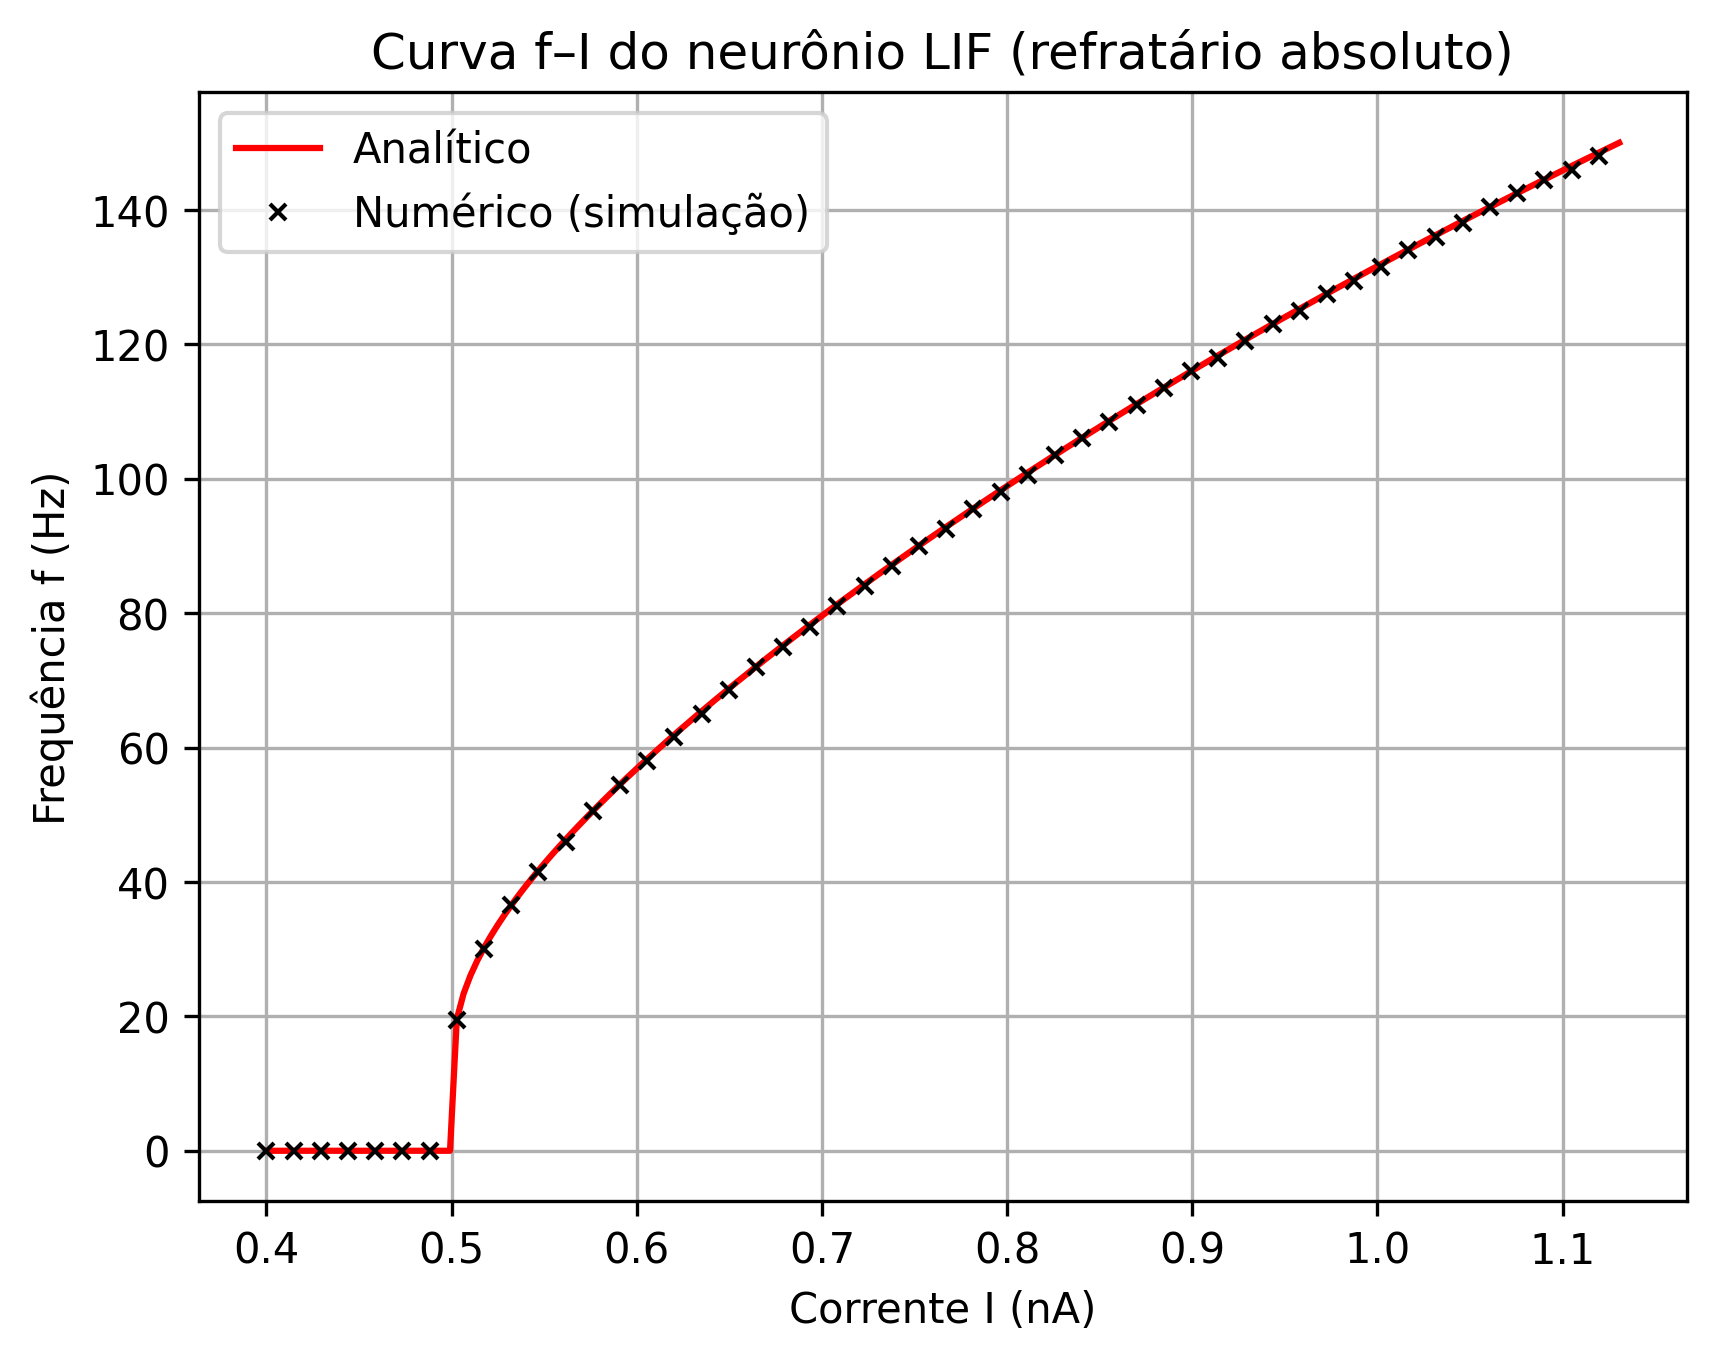
\includegraphics[width=11cm]{../figures/ex_1a.png}
		\caption{Curva f-I do modelo LIF numérica e analítica.}
	\end{figure}
	
	\noindent\textbf{Questão 2:}
	
	
	\noindent \textbf{(a)} Faça o gráfico de f-I para o modelo com ruído para dois valores diferentes de $\sigma$. Para fazer isso, vá aumentando o valor de $\sigma$ a partir de zero até notar que a curva f-I começa a ficar diferente da curva para $\sigma = 0$. Este será o seu primeiro valor de $\sigma$. Depois, continue aumentando $\sigma$ até notar outra mudança significativa na curva f-I. Este será o seu segundo valor de $\sigma$. Apresente os gráficos de f-I para os dois valores de $\sigma$ e explique o que é observado.
	\\
	
	\noindent\textbf{Resposta:}
	
	\begin{figure}[H]
		\centering
		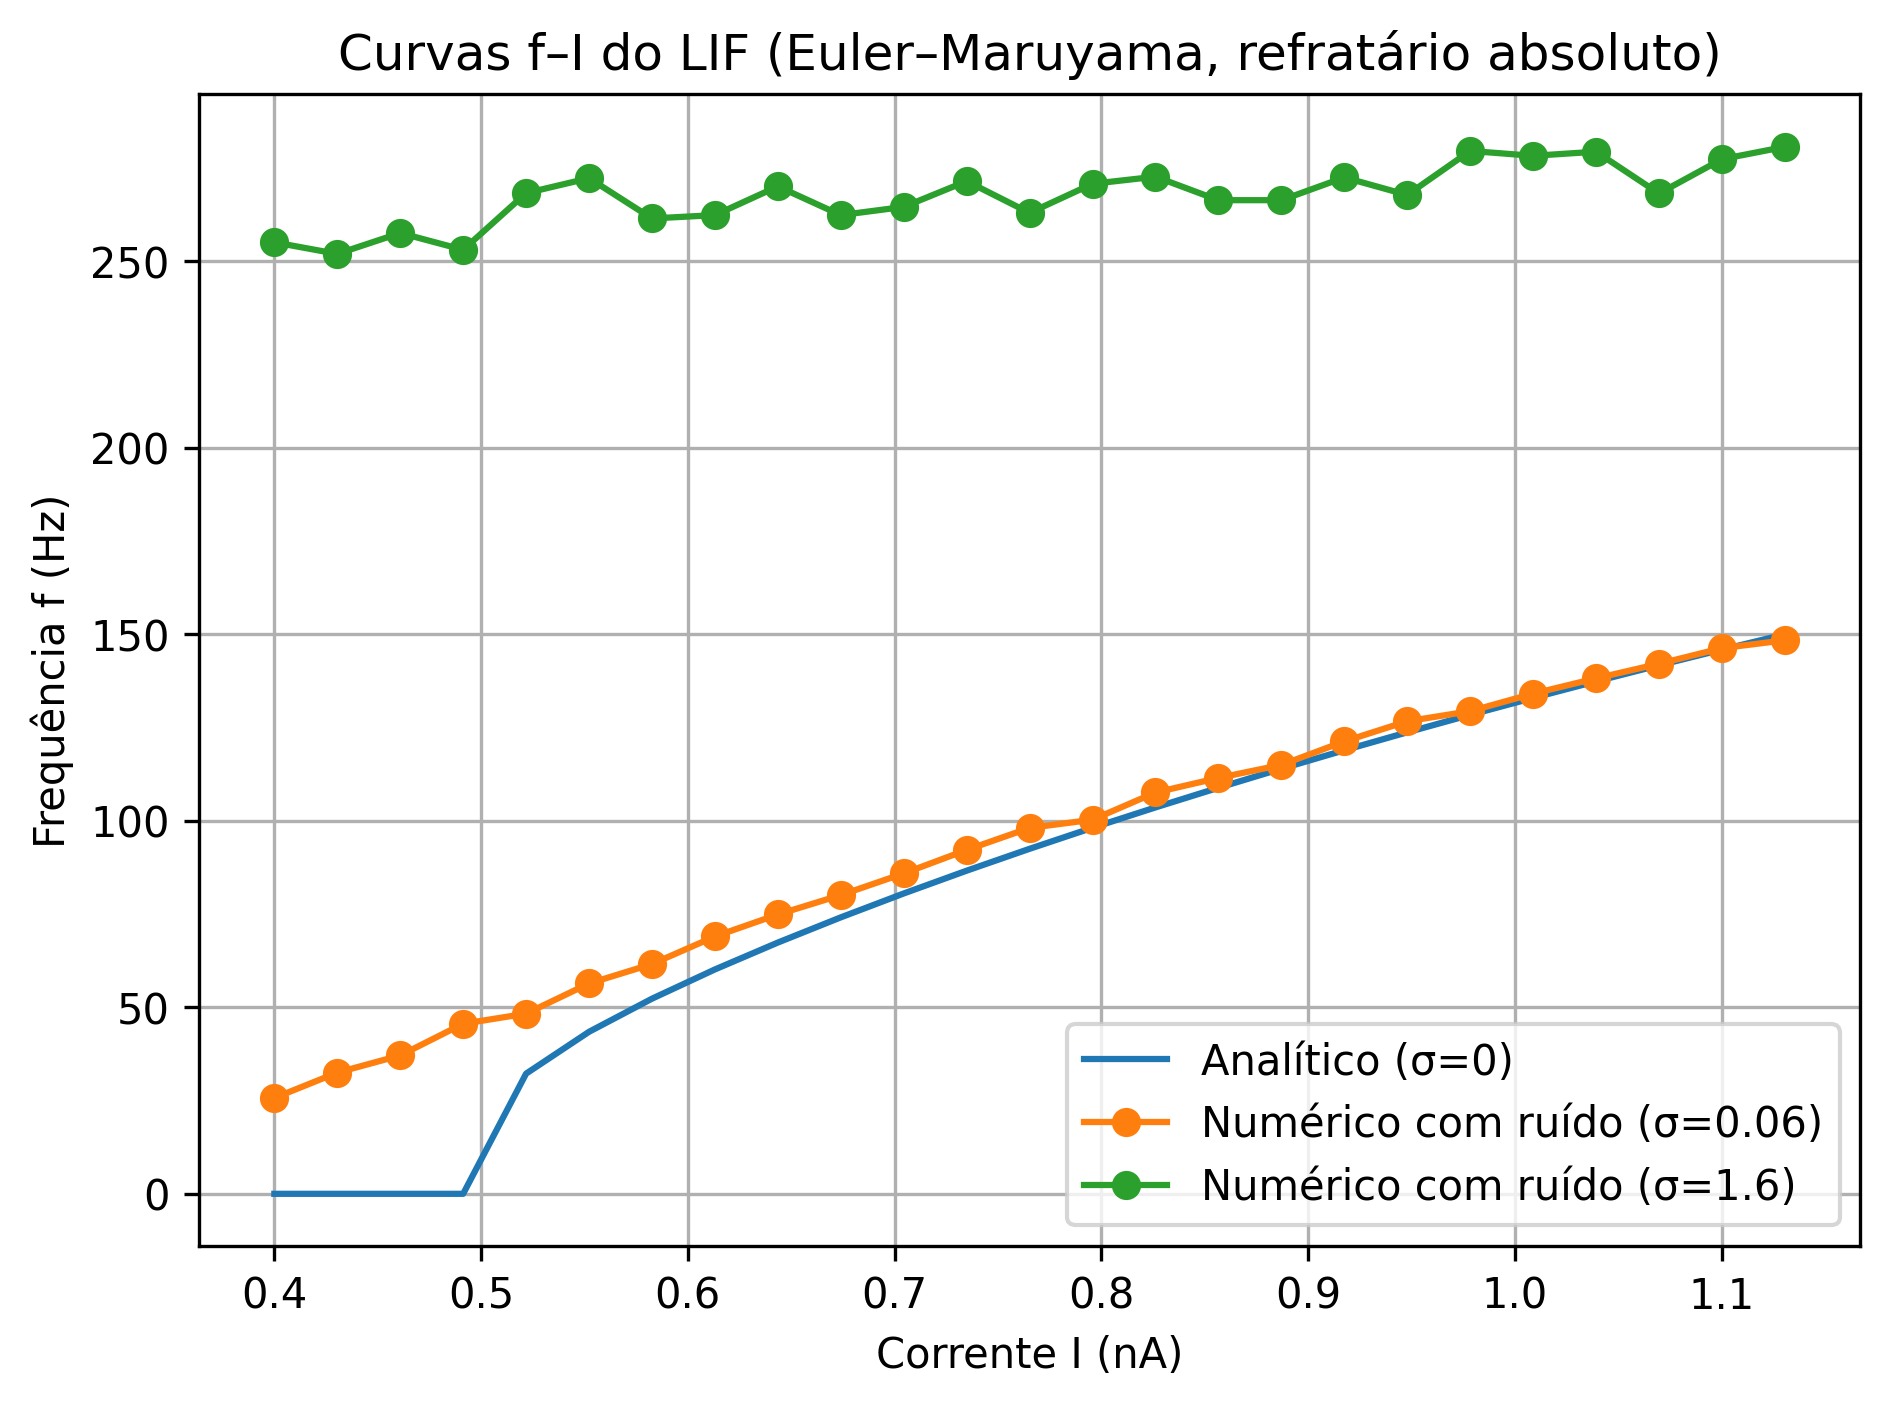
\includegraphics[width=11cm]{../figures/ex_2a.png}
		\caption{Curva f-I do modelo LIF com ruído de diferentes intensidades.}
	\end{figure}
	
	O primeiro efeito do aumento da intensidade do ruído é a antecipação do começo dos disparos; isto é, o neurônio tem frequência não nula para valores em que antes não tinha. O segundo efeito é o apagamento da dependência da frequência com a corrente, tornando-a uma praticamente uma constante ruidosa.\\\\
	
	\noindent \textbf{(b)} Nos comentários relacionados à equação (8.8) de seu livro, Gerstner \textit{et al.} dizem que, independentemente da amplitude do ruído, a trajetória da voltagem $V(t)$ para um dado valor de $I$ torna-se suave quando $\Delta t \to 0$. Faça um estudo do efeito do tamanho do passo de tempo $\Delta t$ sobre a “rugosidade” da trajetória sublimiar de $V(t)$. Para isso, escolha um valor fixo de $I$ que não seja suficiente para fazer que o neurônio sem ruído dispare (por exemplo, $I = 300\,\text{pA}$) e gere diferentes trajetórias de $V(t)$ para um mesmo valor de $\sigma$ (pode ser um dos dois valores que você usou no item anterior). Cada uma das trajetórias deve ser obtida integrando a equação (3) com um passo de tempo $\Delta t$ cada vez menor (comece com o valor de $\Delta t$ usado no item anterior e vá diminuindo por fatores de 10: $\Delta t / 10$, $\Delta t / 100$, $\ldots$, tente ir até o menor valor de $\Delta t$ que você conseguir). Mostre todas as trajetórias obtidas em um mesmo gráfico, com uma cor diferente para cada traçado. O que você pode concluir de seu resultado?\\
	
	\noindent\textbf{Resposta:}
	
	\begin{figure}[H]
		\centering
		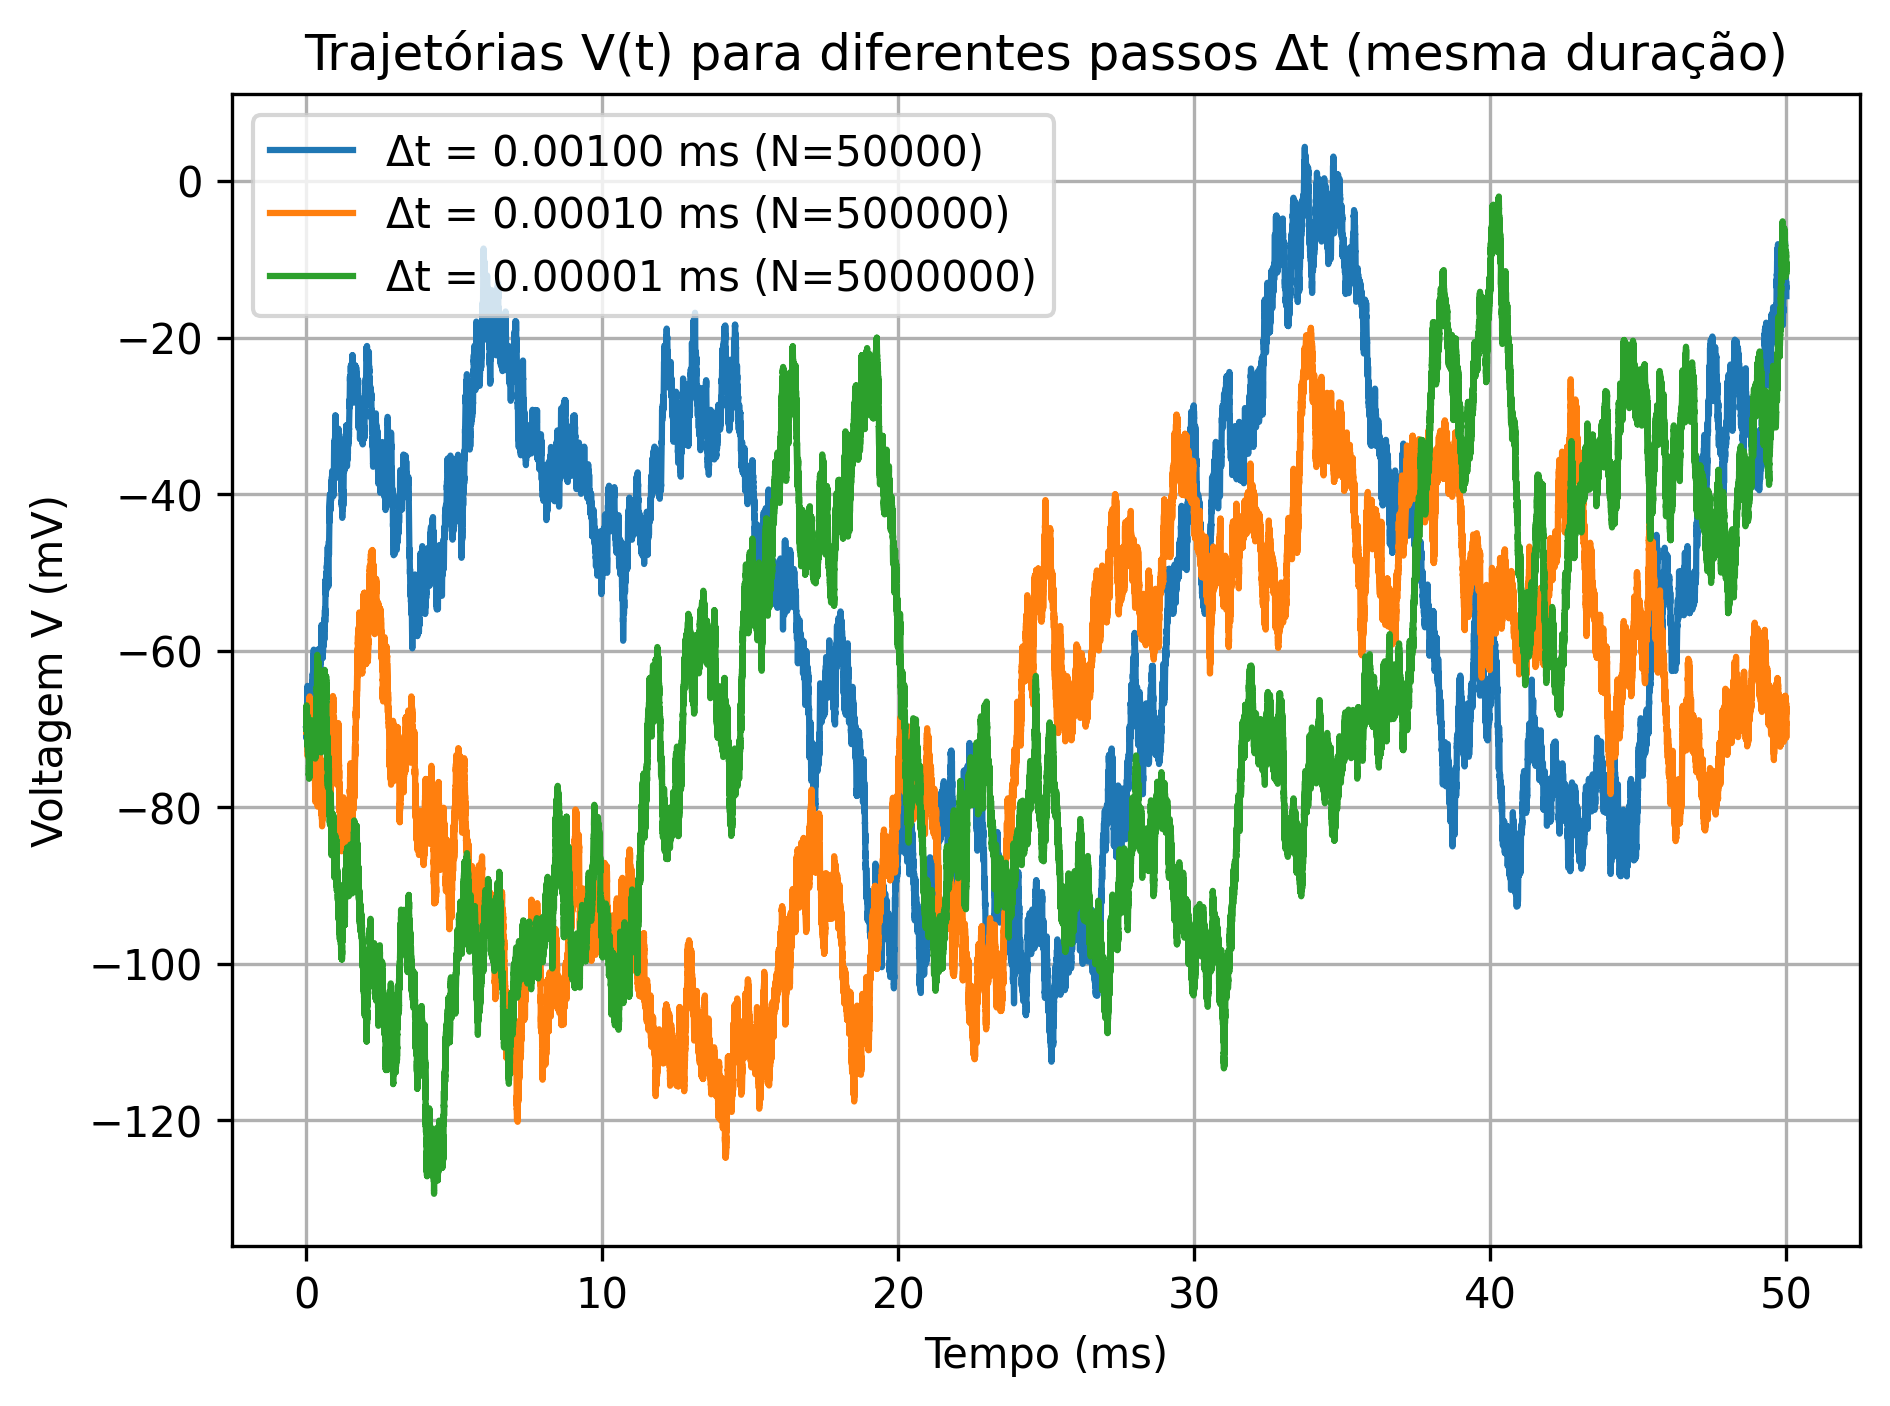
\includegraphics[width=11cm]{../figures/ex_2b.png}
		\caption{Trajetória de $V$ do modelo LIF com ruído para diferentes valores de $\Delta t$.}
	\end{figure}
	
	Aparentemente não houve diferença de rugosidade nas trajetórias para diferentes $\Delta t$.\\\\
	
	\noindent \textbf{(c)} A irregularidade do trem de disparos de um neurônio pode ser quantificada de diferentes maneiras. Uma delas é pelo coeficiente de variação dos intervalos entre disparos, $CV_{\text{ISI}}$, definido como o desvio padrão dos ISIs dividido pela média dos ISIs. Para um neurônio hipotético cujos disparos seguem um processo de Poisson homogêneo, pode-se mostrar que a distribuição dos intervalos entre disparos é exponencial e que $CV_{\text{ISI}} = 1$. Um neurônio desse tipo, chamado de neurônio \textit{poissoniano}, é normalmente usado como controle para comparação com outros modelos de neurônios. Quanto mais próximo de 1 for o $CV_{\text{ISI}}$ do modelo de neurônio, mais próximo ele estará de neurônio poissoniano e mais irregulares serão os seus disparos. Escolha um valor grande para a amplitude do ruído $\sigma$ (por exemplo, o segundo valor do item \textbf{(a)}) e rode a simulação de seu modelo de neurônio com ruído por 2 s com dois valores diferentes de corrente constante $I$ (e mesmo valor de $\sigma$): um acima de $I_L$ (vamos chamá-lo de $I_{\text{acima}}$) e outro abaixo de $I_L$ (vamos chamá-lo de $I_{\text{abaixo}}$), onde $I_L$ é a corrente limiar para o caso sem ruído. Por exemplo, use $I_{\text{acima}} = 570\,\text{pA}$ e $I_{\text{abaixo}} = 430\,\text{pA}$. Gere gráficos para os dois casos como na Figura 5.21 do livro de Dayan e Abbott (pg. 190) citada nas referências da disciplina, no arquivo de roteiro (um pdf do livro foi colocado no Google Sala de Aula). Para cada caso, gere dois gráficos de $V \times t$, um em cima do outro. Coloque no gráfico superior a curva de $V(t)$ sem considerar que o neurônio emite disparos quando a curva cruza o limiar (mecanismo de geração de disparos “desligado”); represente também neste gráfico o limiar de disparo por uma linha horizontal traçada. No gráfico inferior, plote a curva de $V(t)$ usual (com o mecanismo de geração de disparos “ligado”), isto é, com os disparos postos à mão quando a voltagem atinge ou ultrapassa o limiar vindo de baixo. Use as mesmas escalas (aquelas que mostram os disparos) para ambos os gráficos. Faça isso para os dois casos e, a partir deles, os ISIs respectivos. Tendo os ISIs, calcule o valor médio e o desvio padrão e obtenha o $CV_{\text{ISI}}$ para cada caso. Como se comportam? Em qual dos dois casos os disparos do neurônio são mais regulares? Explique o porquê da diferença observada (para isso, será útil ler a Seção \textit{Regular and Irregular Firing Models} do livro de Dayan e Abbott (pgs. 189–191). Nota: dependendo do valor de $\sigma$ usado, os disparos podem não ficar exatamente como na Figura 5.21 do livro de Dayan e Abbott. Tente gerar gráficos mais ou menos parecidos com os da Figura 5.21 do livro de Dayan e Abbott.
	\\
	
	\noindent\textbf{Resposta:}
	
	\begin{figure}[H]
		\centering
		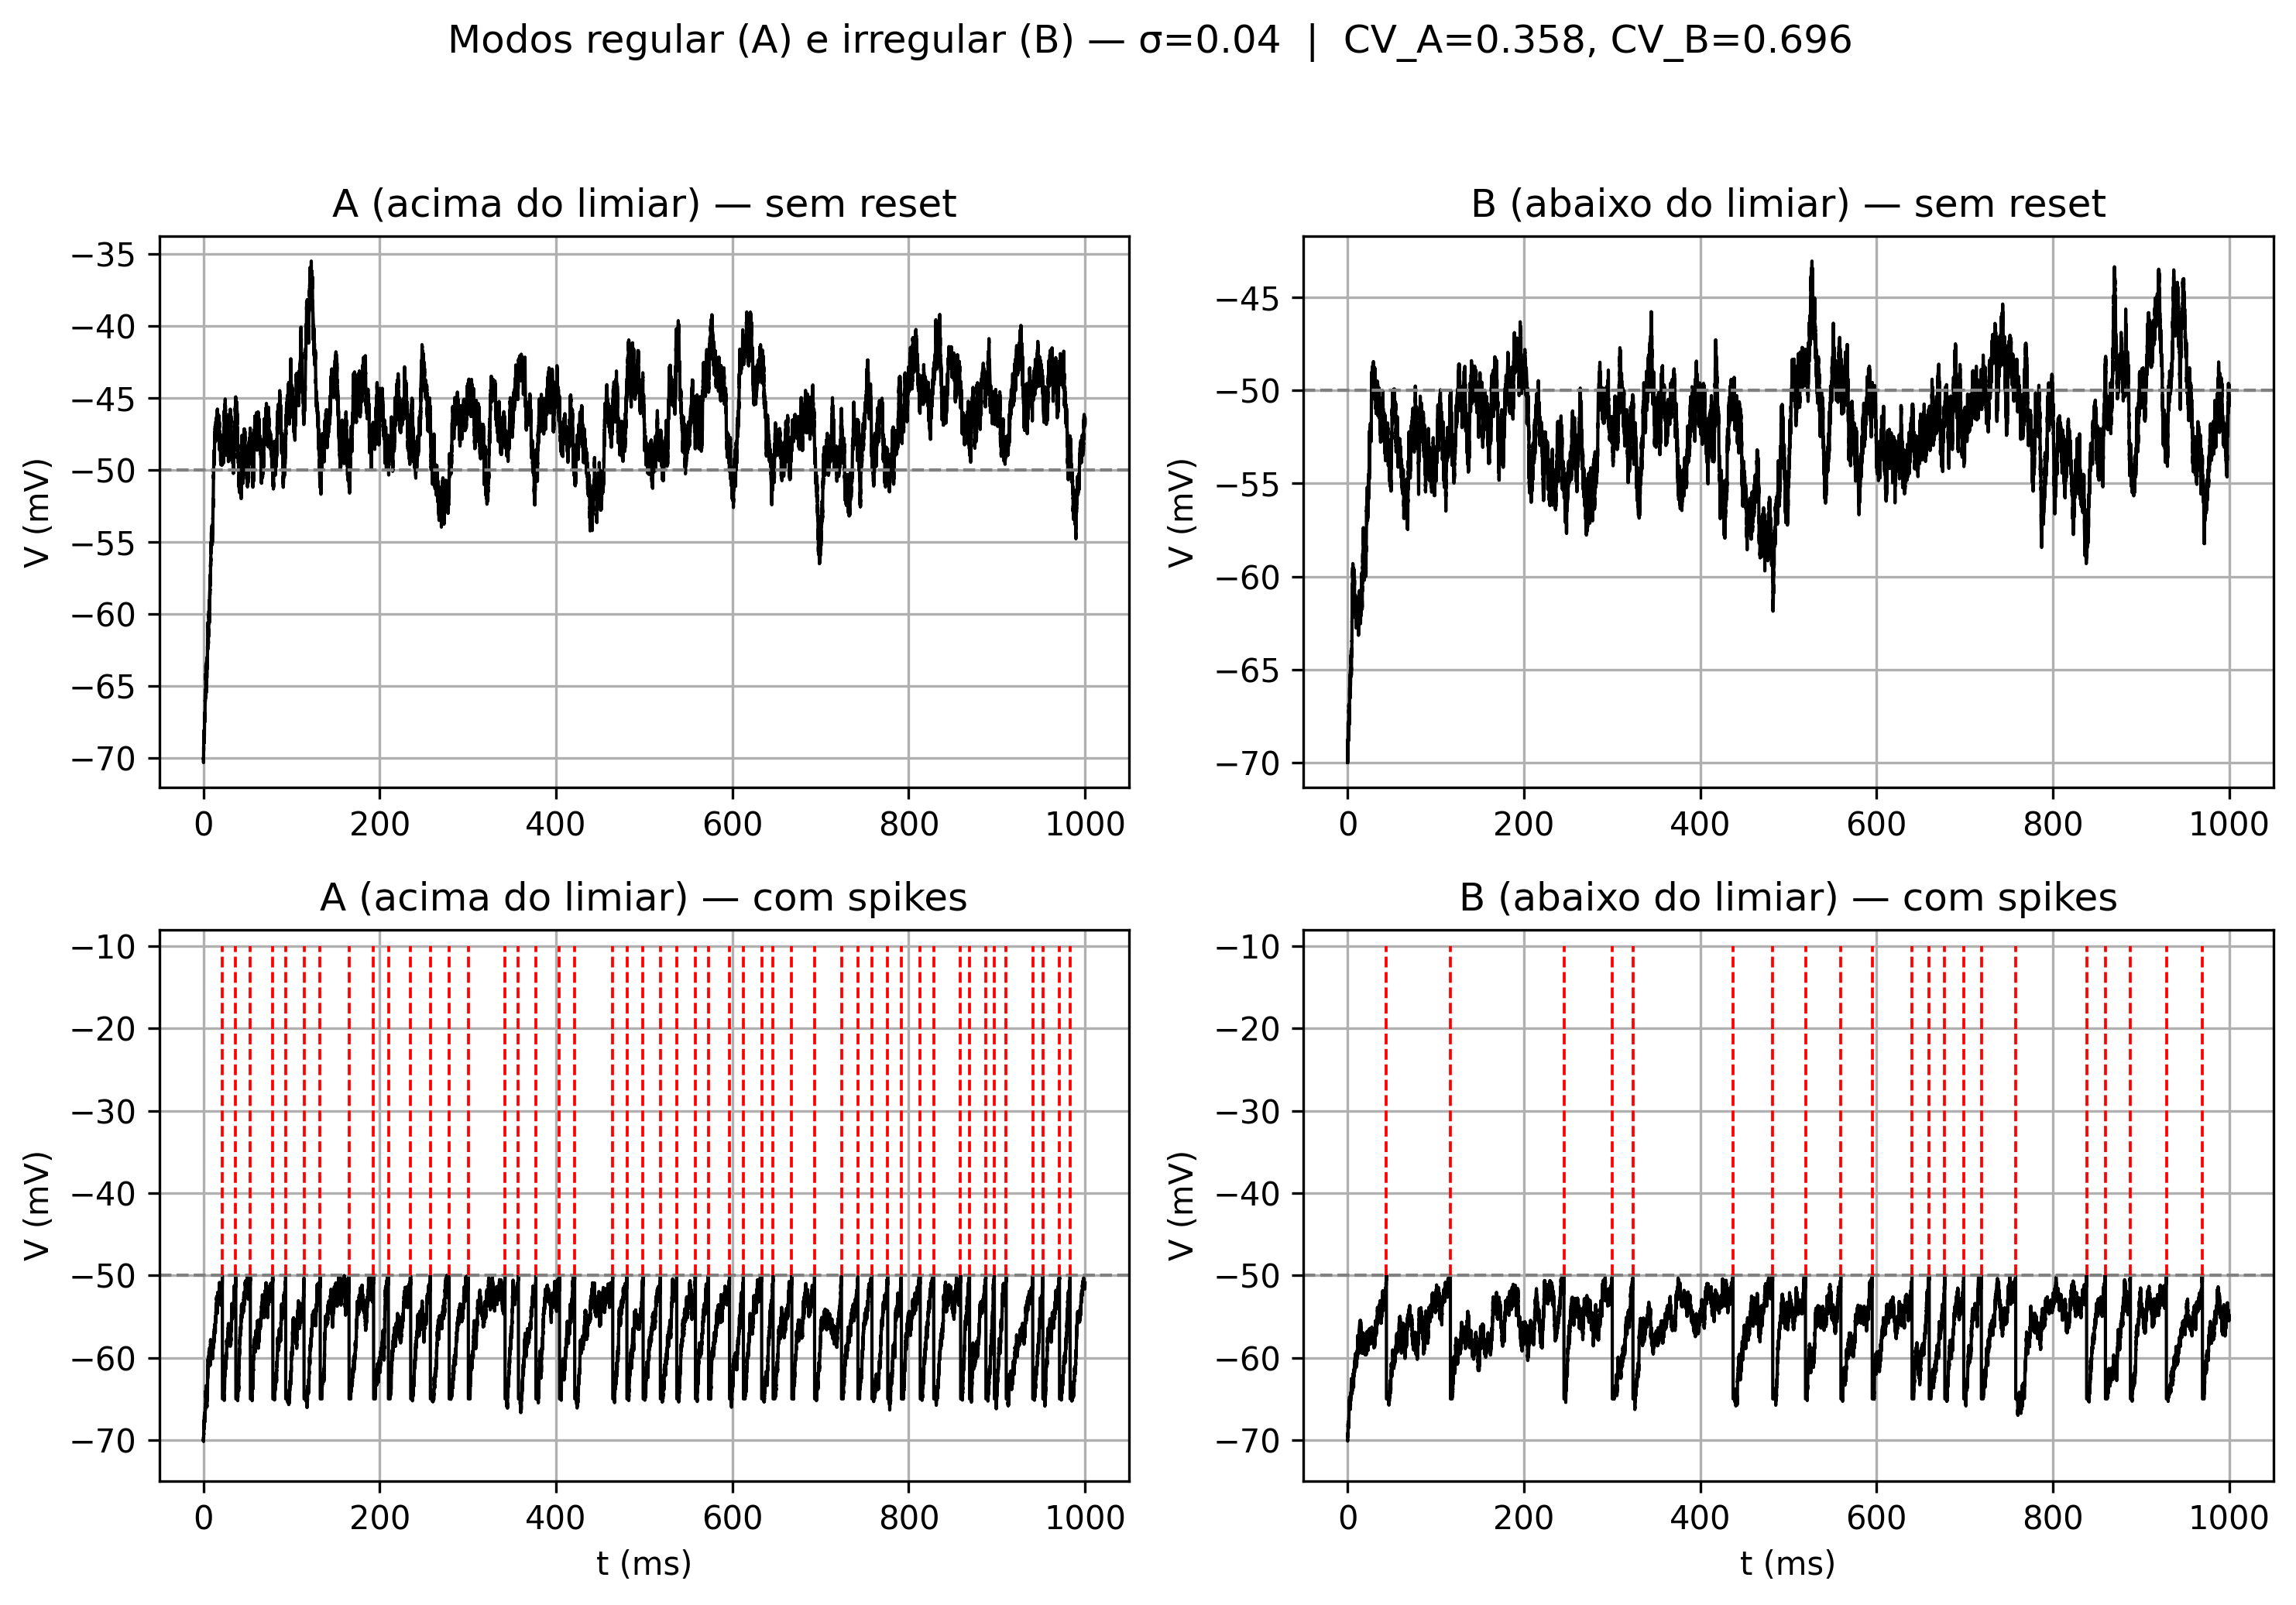
\includegraphics[width=11cm]{../figures/ex_2c.png}
		\caption{Trem de disparos regular e irregular do modelo LIF com ruído devido a diferentes correntes aplicadas.}
	\end{figure}
	
	No caso A os disparos parecem ser menos aleatórios e mais consistentes, enquanto no caso B parece imprevisível. O valor de CV para cada caso está na figura. O CV no caso B é praticamente o dobro, indicando alta irregularidade; compatível com o que observamos qualitativamente na figura. Este fenômeno acontece porque, para a corrente acima do limiar, o efeito do ruído em $V$ fica quase todo acima do limiar, e acaba não influenciando no tempo de disparo: o comportamento pode ser aproximado por uma corrente constante acima do limiar; e no caso em que a corrente está abaixo do limiar, o ruído tem forte influência em quando $V$ vai superar o limiar, refletindo sua característica estocástica nos instantes irregulares que o neurônio dispara.\\\\
	
	\noindent\textbf{Questão 3:}
	

	\noindent \textbf{(a)} Simule o modelo de neurônio por $1{,}5 \ \text{s}$ com um pulso de corrente $I = 501 \ \text{pA}$ aplicado de $t = 0{,}5 \ \text{s}$ a $t = 1{,}0 \ \text{s}$. Coloque os seus resultados em uma figura composta por três gráficos, um dando a corrente aplicada $I$ em função do tempo, outro dando o potencial de membrana $V$ em função do tempo, e o terceiro dando a condutância de adaptação $G_a$ em função do tempo. Faça com que os gráficos fiquem um em cima do outro para facilitar a comparação.
	\\
	
	\noindent\textbf{Resposta:}
	
	\begin{figure}[H]
		\centering
		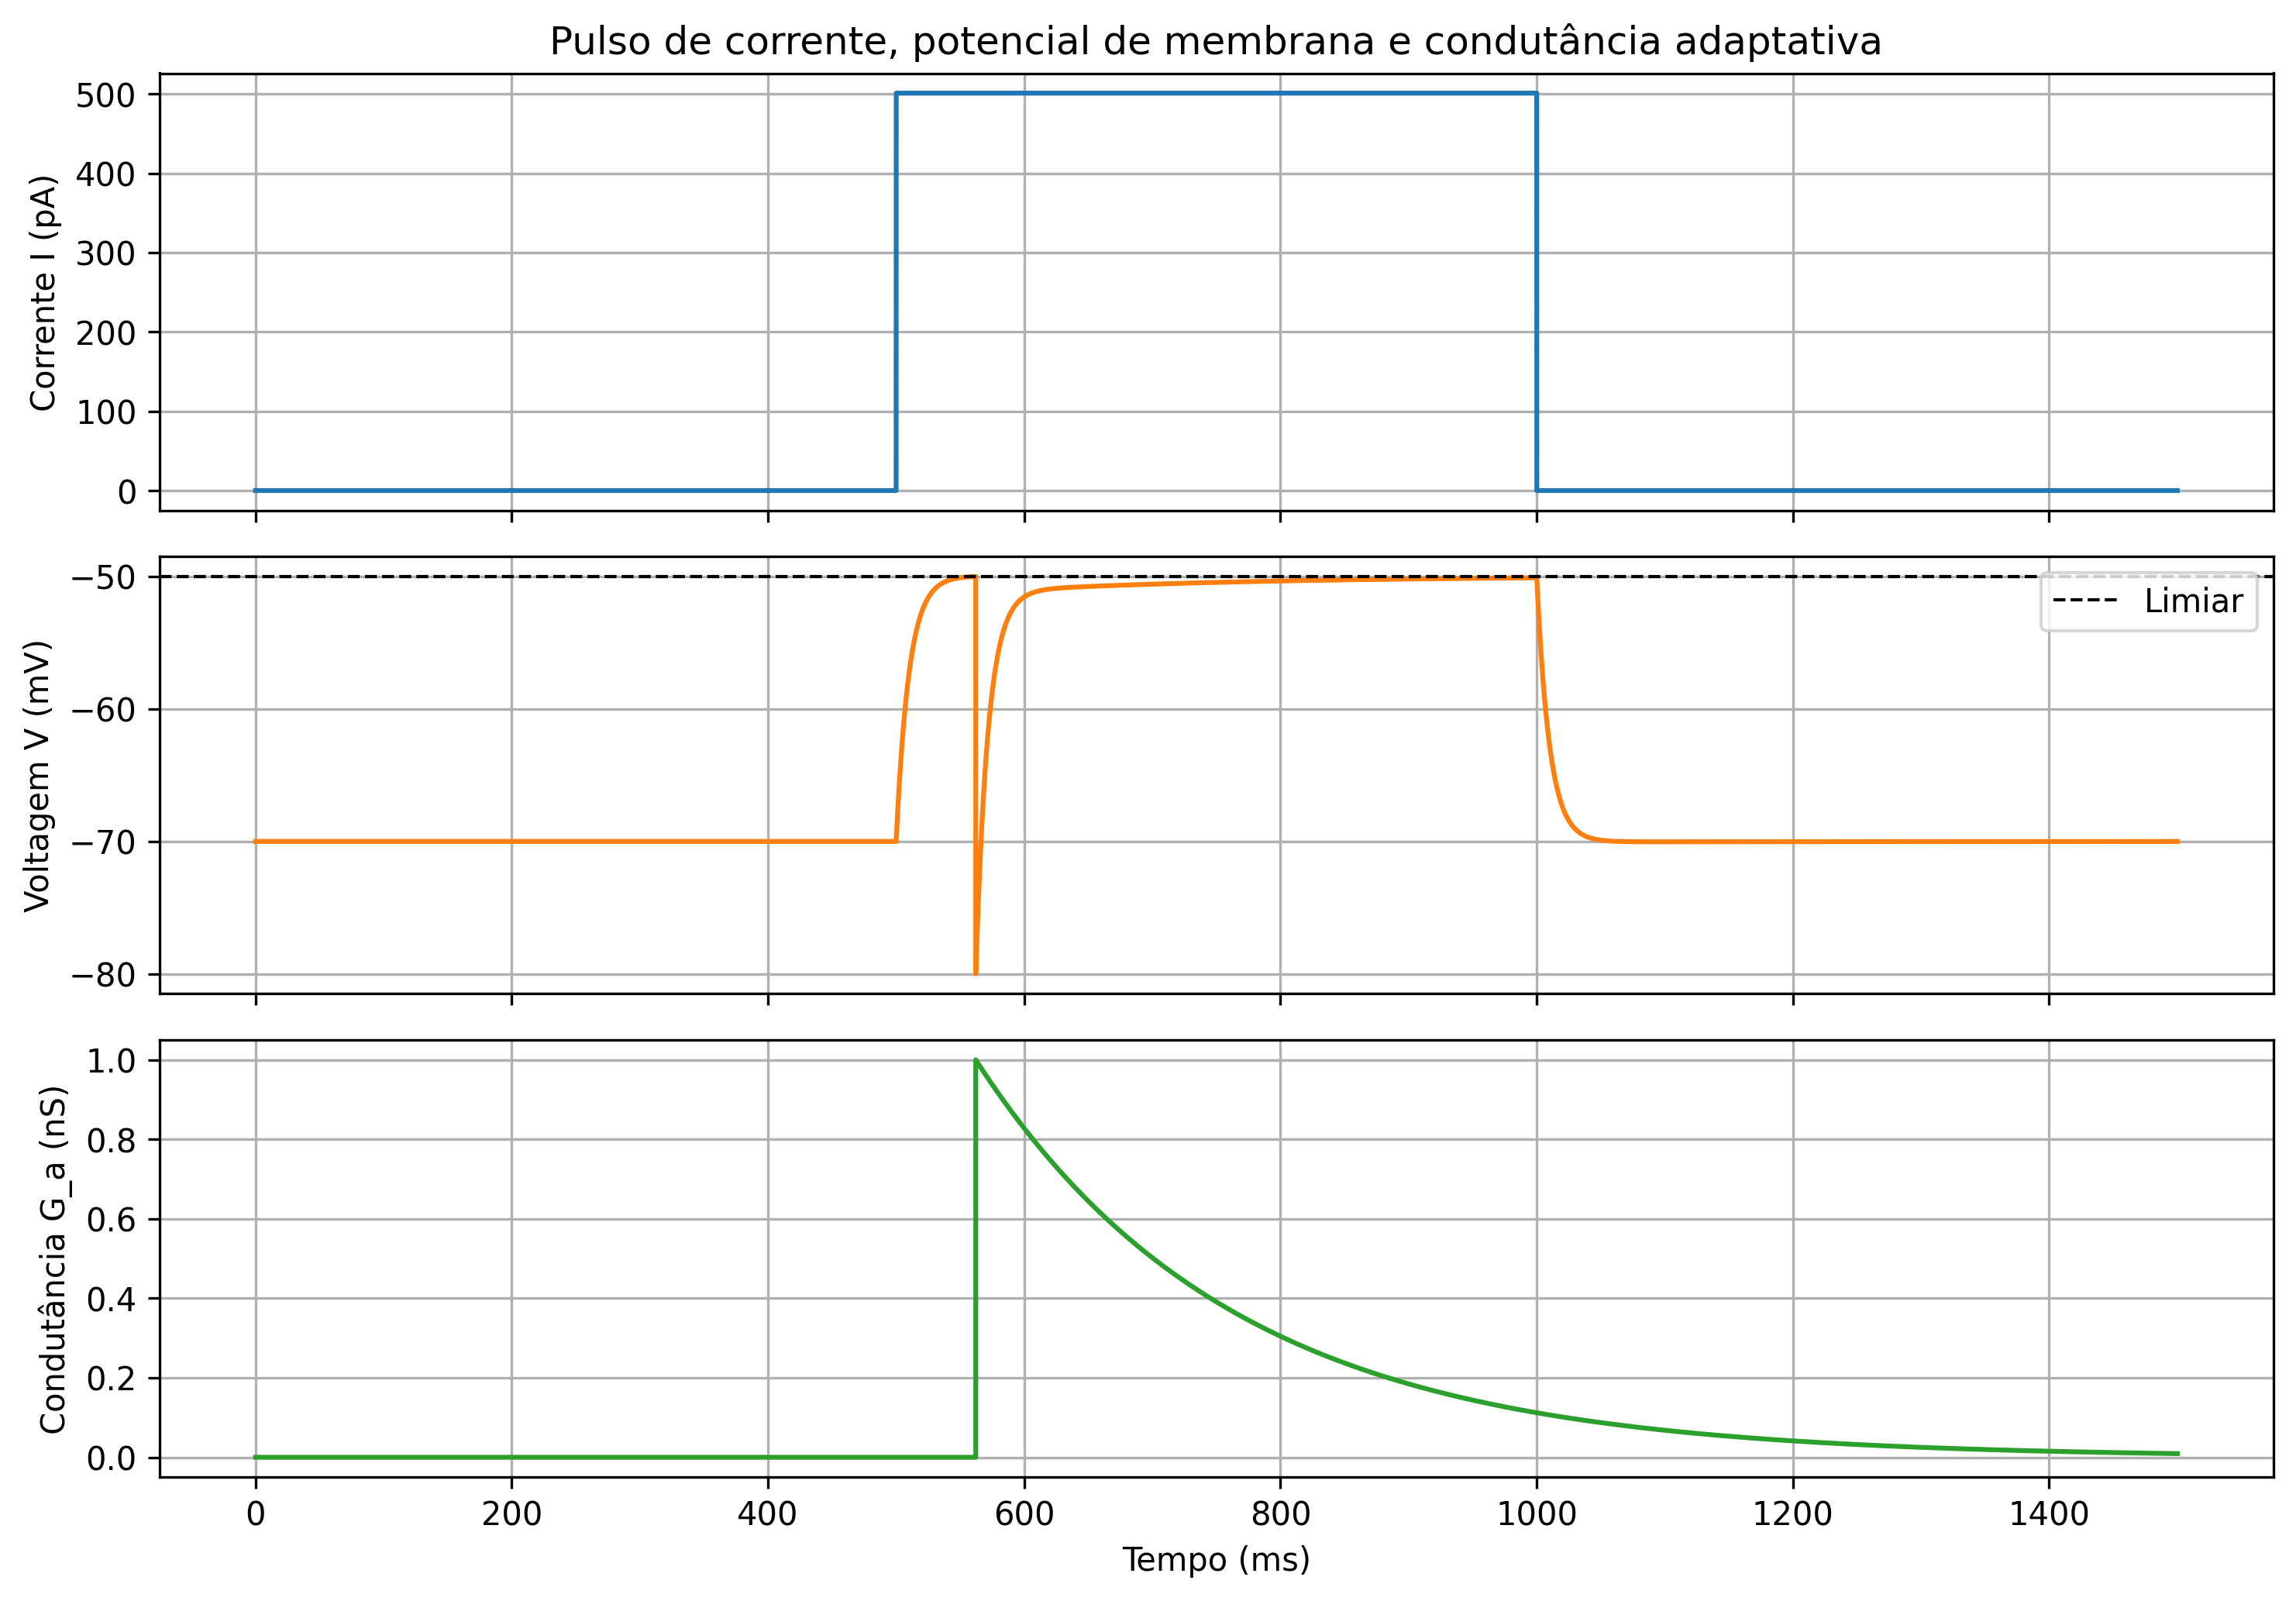
\includegraphics[width=11cm]{../figures/ex_3a.png}
		\caption{Dinâmica do modelo LIF com corrente adaptativa.}
	\end{figure}
	
	
	\noindent \textbf{(b)} Agora simule o modelo por $5 \ \text{s}$ usando diferentes valores de corrente injetada constante $I$, indo de $I = 400 \ \text{pA}$ a $I = 800 \ \text{pA}$ em incrementos de $20 \ \text{pA}$. Para cada corrente aplicada, calcule o primeiro intervalo entre disparos ($T_1 = t_2 - t_1$ na notação das notas de aula) e o intervalo entre disparos do regime estacionário (isto é, depois do período transiente) $T_\infty$. Faça um gráfico mostrando as curvas f-I obtidas pelo inverso de $T_1$ ($f_1$) e pelo inverso de $T_\infty$ ($f_\infty$), representadas por símbolos ou cores diferentes. O modelo simulado é de tipo I ou de tipo II?\\
	
	\noindent\textbf{Resposta:}
	
	\begin{figure}[H]
		\centering
		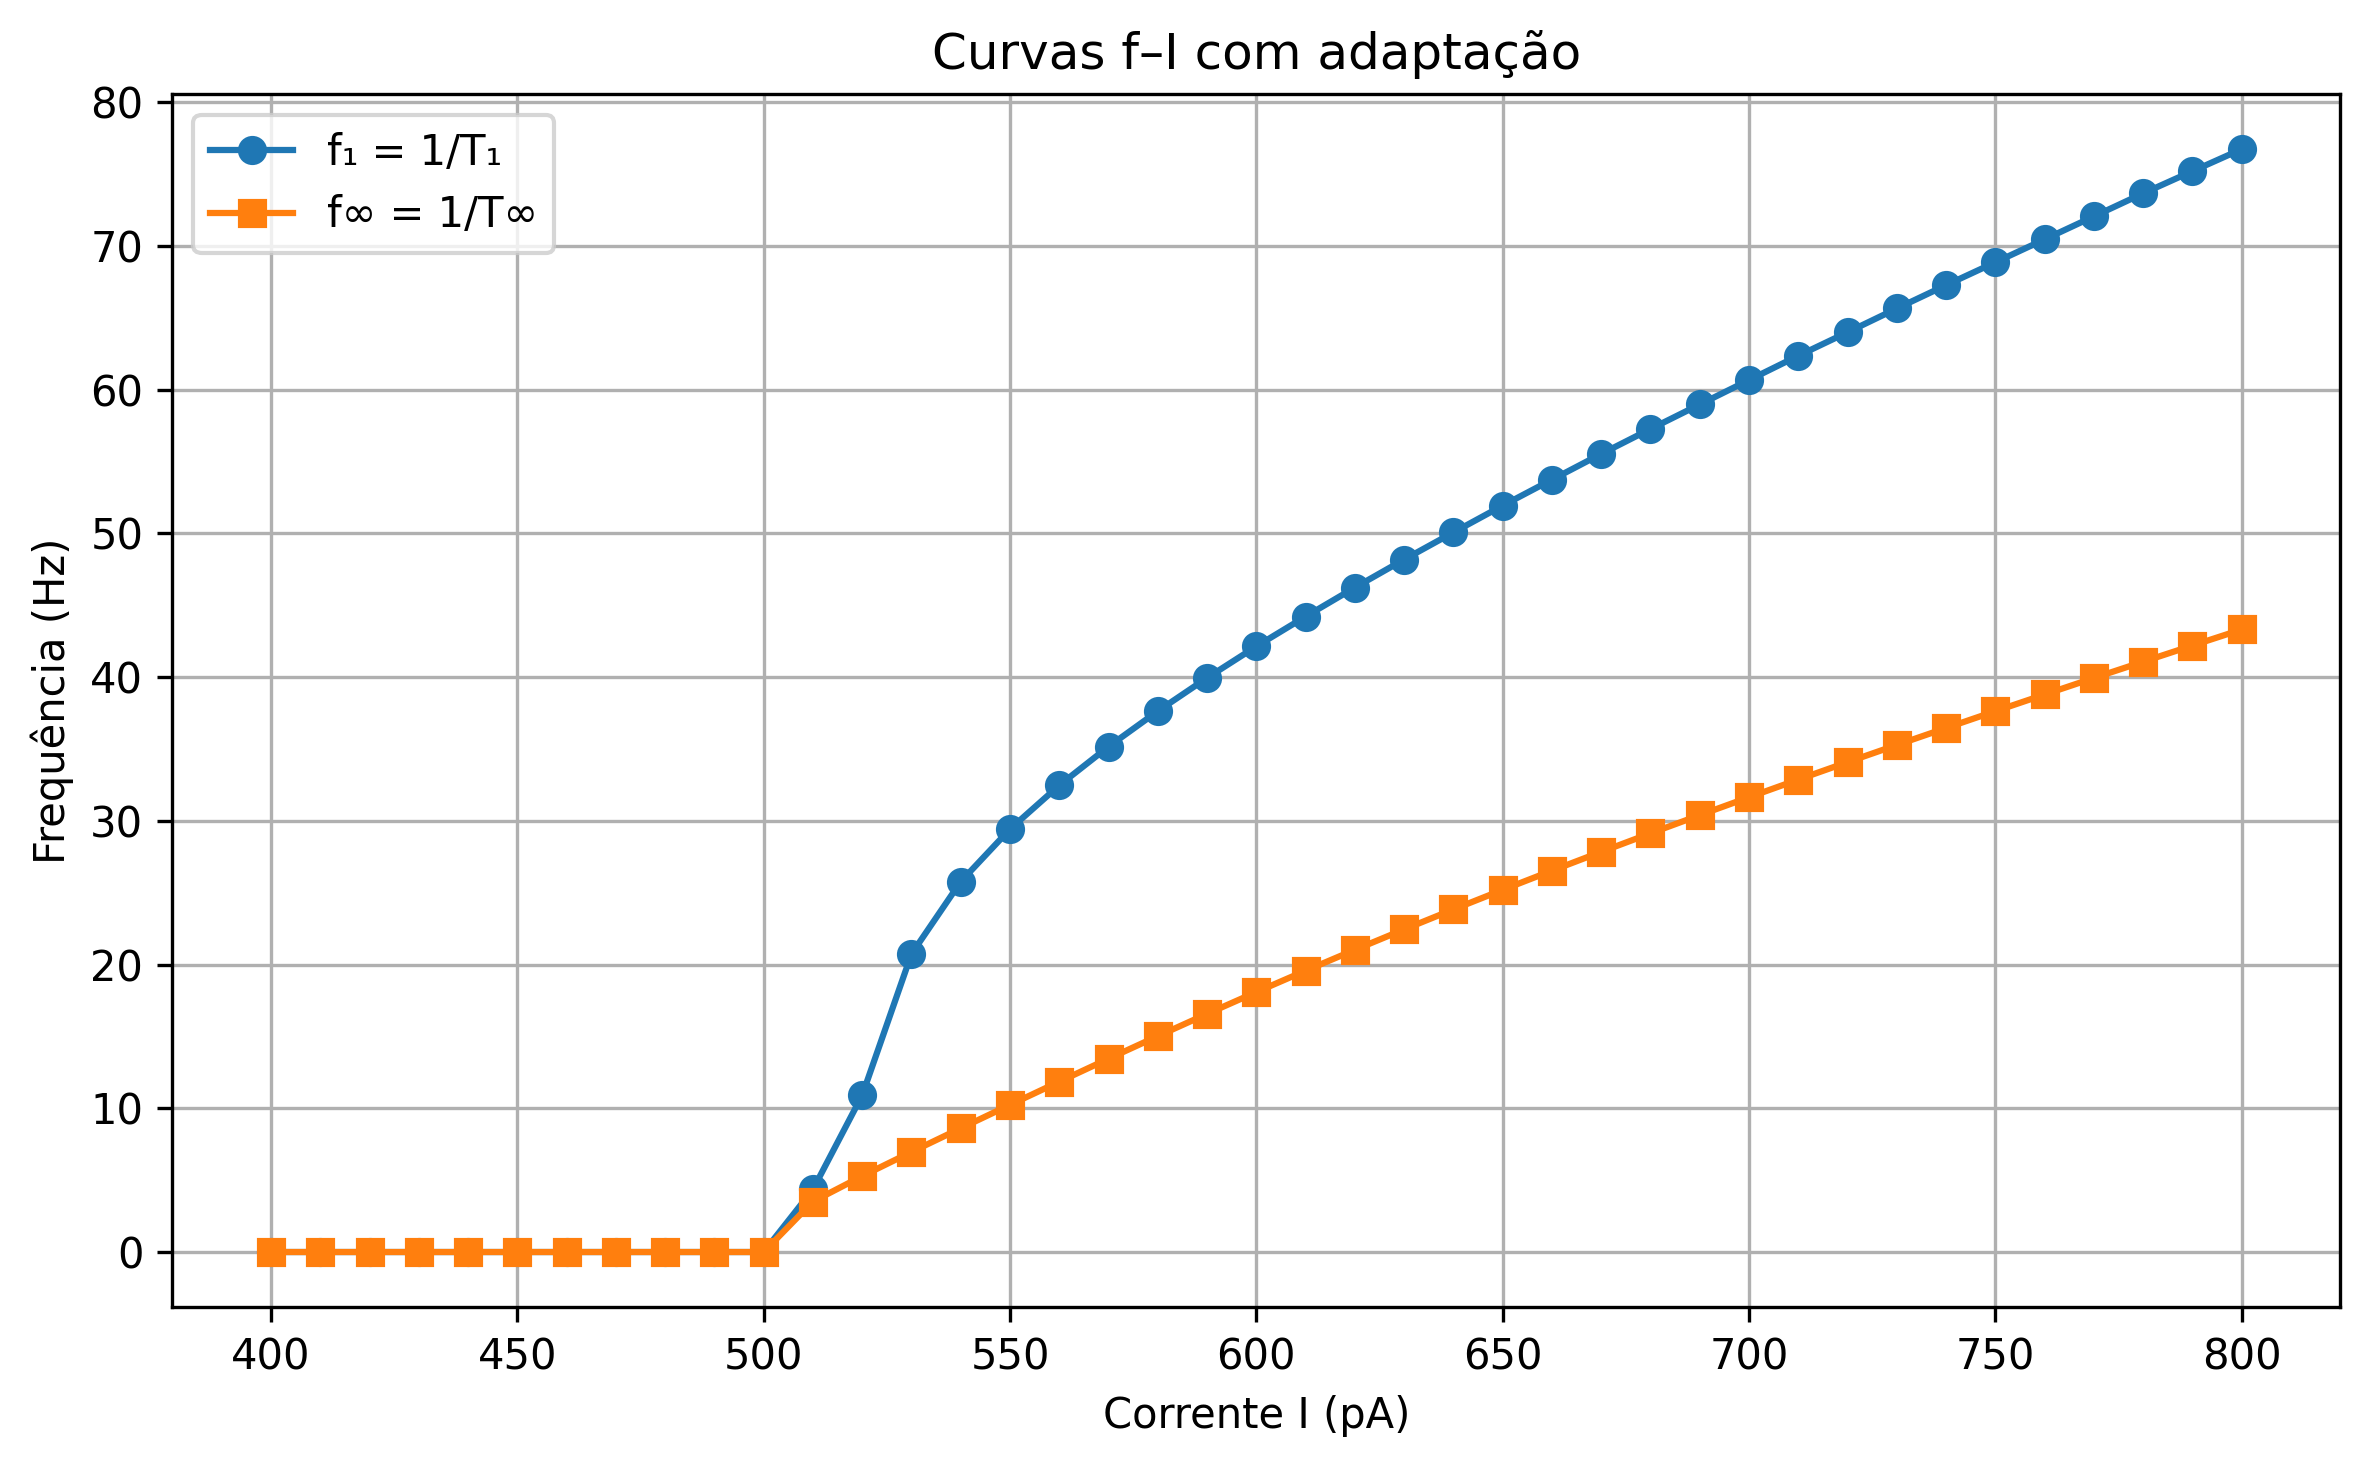
\includegraphics[width=11cm]{../figures/ex_3b.png}
		\caption{Curvas f-I do modelo LIF com corrente adaptativa.}
	\end{figure}
	
	O modelo aparenta ser de tipo I, apesar de a curva obtida por $T_1$ ter um comportamento esquisito perto da corrente de reobase.
	
\end{document}